\documentclass[11pt,a4paper]{article}

\usepackage[T1]{fontenc}
\usepackage{lmodern}
\usepackage[a4paper,left=22mm,right=22mm,top=23mm,bottom=22mm,headheight=15pt]{geometry}
\usepackage{graphicx}
\usepackage{array}
\usepackage{tabularx}
\usepackage{booktabs}
\usepackage{longtable}
\usepackage{enumitem}
\usepackage{fancyhdr}
\usepackage{titlesec}
\usepackage{caption}
\usepackage{subcaption}
\usepackage{microtype}
\usepackage{amsmath}
\usepackage{amssymb}
\usepackage{float}
\usepackage{xcolor}
\usepackage{tikz}
\usetikzlibrary{arrows.meta,positioning,calc}
\usepackage[hidelinks]{hyperref}
\usepackage{url}

\graphicspath{{../figures/jpg/}}
\setlength{\parindent}{0pt}
\setlength{\parskip}{5pt}
\setlength{\emergencystretch}{2em}
\raggedbottom
\urlstyle{same}

\setlist[itemize]{leftmargin=5.5mm,itemsep=1.5pt,topsep=3pt,parsep=0pt}
\setlist[enumerate]{leftmargin=7mm,itemsep=1.5pt,topsep=3pt,parsep=0pt}

\titleformat{\section}{\normalfont\Large\bfseries}{\thesection.}{0.55em}{}[\vspace{1.5pt}\titlerule]
\titlespacing*{\section}{0pt}{13pt}{6pt}
\titleformat{\subsection}{\normalfont\large\bfseries}{\thesubsection}{0.55em}{}
\titlespacing*{\subsection}{0pt}{8pt}{2pt}
\titleformat{\subsubsection}{\normalfont\normalsize\bfseries}{\thesubsubsection}{0.55em}{}

\captionsetup{font=small,labelfont=bf,textfont=it,justification=centering,skip=5pt}

\pagestyle{fancy}
\fancyhf{}
\fancyhead[R]{\small\bfseries 3D SMART CITY WITH DIGITAL TRAFFIC SIGNALS -- PROJECT REPORT}
\fancyfoot[C]{\thepage}
\renewcommand{\headrulewidth}{0pt}

\newcommand{\code}[1]{\texttt{\small #1}}
\newcommand{\shot}[2]{\includegraphics[width=#1]{#2}}
\newenvironment{calc}[1]{\par\smallskip\noindent\begin{minipage}{\textwidth}\setlength{\fboxsep}{6pt}\begin{lrbox}{0}\begin{minipage}{0.955\textwidth}\textbf{Worked calculation: #1}\par\smallskip}{\end{minipage}\end{lrbox}\fbox{\usebox{0}}\end{minipage}\par\smallskip}

\begin{document}

% =============================================================================
% Cover
% =============================================================================
\thispagestyle{empty}
\begin{center}
  {\Large\bfseries CSE 4102: Graphics Lab\par}
  \vspace{1mm}
  {\normalsize Computer Graphics and Image Processing Laboratory\par}
  \vspace{3mm}
  \rule{\textwidth}{0.8pt}

  \vspace{10mm}
  {\LARGE\bfseries PROJECT REPORT\par}
  \vspace{9mm}
  {\fontsize{26}{31}\selectfont\bfseries 3D Smart City with\\[2mm] Digital Traffic Signals\par}
  \vspace{6mm}
  {\large\bfseries An interactive OpenGL city: traffic, signals, people,\\ day and night, weather and partial ray tracing\par}
  \vspace{4mm}
  \rule{0.70\textwidth}{0.7pt}

  \vspace{8mm}
  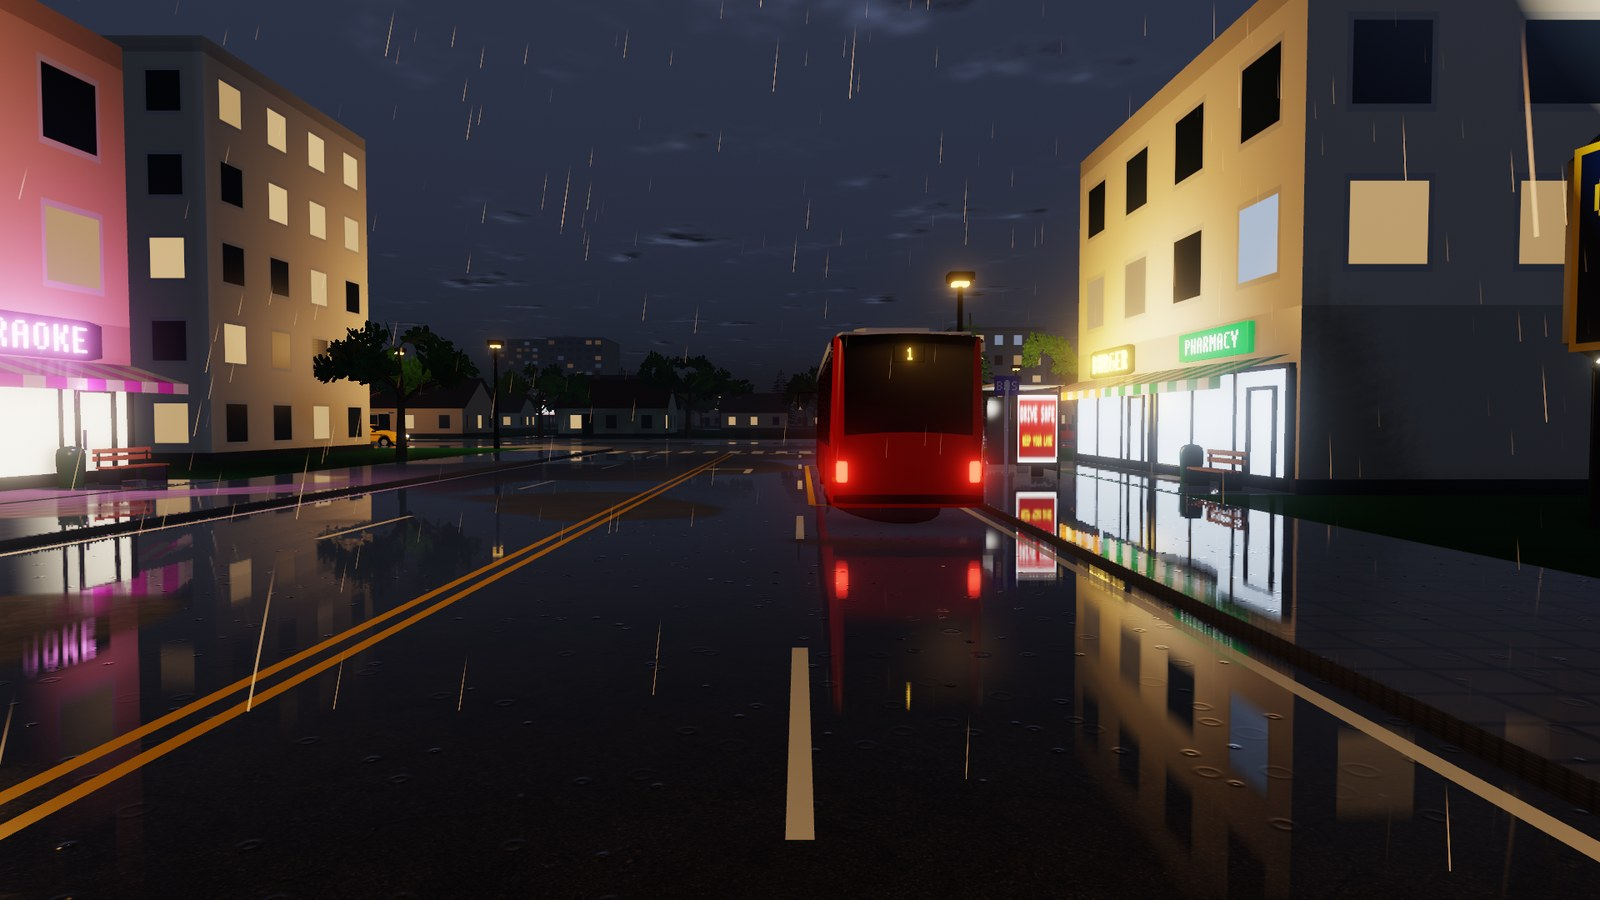
\includegraphics[width=0.92\textwidth]{rt_on_rain_night}

  \vspace{8mm}
  \renewcommand{\arraystretch}{1.45}
  \begin{tabular}{@{}>{\bfseries}p{38mm}@{\hspace{8mm}}p{68mm}@{}}
    Submitted by: & Asif Jawad \\
    Roll:         & 2107007 \\
    Section:      & A \\
    Course:       & CSE 4102: Graphics Lab \\
    Date:         & 26 September 2026
  \end{tabular}
\end{center}
\vfill
\newpage

\tableofcontents
\newpage

% =============================================================================
\section{Introduction}
% =============================================================================

\textbf{3D Smart City with Digital Traffic Signals} is an interactive city simulation written in C++ with modern OpenGL~3.3 (core profile). A closed city 400\,m across holds 19 junctions of five kinds, 36 vehicles of 11 kinds that obey digital traffic signals, 80 people who wait for the walk lights and cross, 164 buildings, 255 trees and a full day--night cycle with weather. The user can fly a free camera, look down from above, follow any car, or drive a car of their own from a chase view or from the driver's seat, and get out and walk.

Every object in the scene is authored geometry: there is no imported model file anywhere. Buildings are boxes whose windows are drawn by the fragment shader; the fountain, lamp posts, bins and bollards are Bezier surfaces of revolution; vehicle bodies are lofted from Bezier profiles; trees are tubes swept along 3D Bezier curves with alpha-tested leaf cards.

\noindent\fbox{\parbox{0.965\textwidth}{%
\textbf{Lab topics shown in this project}\par
\begin{itemize}
  \item \textbf{2D and 3D transformations:} model, view and projection matrices; routes rotated and translated onto every junction; hierarchical vehicles with wheels that roll by $\Delta\theta = d/r$.
  \item \textbf{Illumination model:} ambient + diffuse + specular with a \textbf{directional} light (sun and moon), \textbf{point} lights (194 lamps), \textbf{spot} lights (a billboard lamp and headlights) and \textbf{emissive} surfaces (neon, windows, signals).
  \item \textbf{Shading:} flat, Gouraud and Phong, switchable while it runs (keys \code{1}, \code{2}, \code{3}).
  \item \textbf{Texture mapping:} diffuse and specular maps, wrapping and filtering modes, alpha-tested leaves.
  \item \textbf{Curves and surfaces:} Bezier curves and surfaces of revolution.
  \item \textbf{Ray tracing (bonus):} partial ray tracing through the depth buffer: reflections, ambient occlusion, contact shadows, soft shadows and sun shafts.
\end{itemize}}}

\subsection{Objectives}
\begin{enumerate}
  \item Build a believable 3D city entirely from code, with every object's size taken from real-world measurements.
  \item Show every topic of the lab clearly: transformations, the illumination model with each light type, the three shading modes, textures, Bezier curves, and ray tracing.
  \item Simulate traffic that is \emph{collision-free by construction} and obeys digital signals, with pedestrians who cross safely.
  \item Keep the frame rate steady at 1920$\times$1080 (72\,FPS on the test laptop), with no judder.
\end{enumerate}

\begin{figure}[H]
  \centering
  \begin{subfigure}{0.49\textwidth}\shot{\textwidth}{city_overview}\caption{The whole city at 15:30}\end{subfigure}\hfill
  \begin{subfigure}{0.49\textwidth}\shot{\textwidth}{top_view}\caption{Top view (\code{M})}\end{subfigure}
  \caption{The closed 400\,m city: a core of six junctions inside a ring road.}
\end{figure}

% =============================================================================
\section{System Overview}
% =============================================================================

\subsection{Tools}
\begin{tabularx}{\textwidth}{@{}>{\bfseries}l X@{}}
Language & C++20, Visual Studio 2022+ (MSVC), x64 \\
Graphics & OpenGL 3.3 core profile, GLSL 330 \\
Libraries & GLFW (window, input), GLAD (OpenGL loader), GLM (matrices), stb\_image (textures), stb\_easy\_font (text strokes) \\
GPU used & NVIDIA RTX 3050 laptop GPU, 1920$\times$1080 \\
Code size & about 60 C++ source files and 40 shader files \\
\end{tabularx}

\subsection{Frame pipeline}
Each frame runs the steps below. The simulation always advances in fixed 1/60\,s steps and every frame draws a blend of the last two steps (render interpolation), so motion is the same on any computer and smooth on any screen.

\begin{figure}[H]
\centering
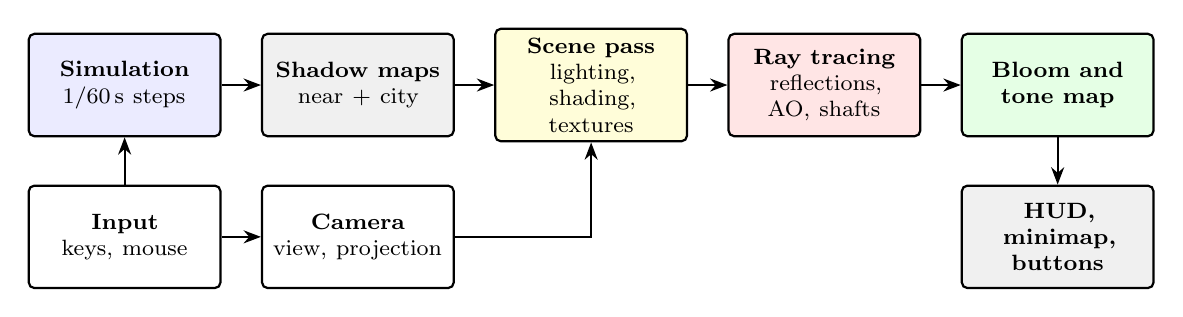
\begin{tikzpicture}[
  box/.style={draw,thick,rounded corners=2pt,align=center,minimum height=13mm,text width=22mm,font=\footnotesize\bfseries,fill=#1},
  box/.default=white,
  arr/.style={-{Stealth[length=2.2mm]},thick}]
  \node[box=blue!8] (sim) {Simulation\\\normalfont 1/60\,s steps};
  \node[box=gray!12,right=5mm of sim] (shadow) {Shadow maps\\\normalfont near + city};
  \node[box=yellow!15,right=5mm of shadow] (scene) {Scene pass\\\normalfont lighting, shading, textures};
  \node[box=red!10,right=5mm of scene] (rt) {Ray tracing\\\normalfont reflections, AO, shafts};
  \node[box=green!10,right=5mm of rt] (post) {Bloom and tone map};
  \node[box=gray!12,below=6mm of post] (hud) {HUD, minimap, buttons};
  \node[box=white,below=6mm of sim] (input) {Input\\\normalfont keys, mouse};
  \node[box=white,right=5mm of input] (cam) {Camera\\\normalfont view, projection};
  \draw[arr] (sim) -- (shadow); \draw[arr] (shadow) -- (scene); \draw[arr] (scene) -- (rt);
  \draw[arr] (rt) -- (post); \draw[arr] (post) -- (hud);
  \draw[arr] (input) -- (sim); \draw[arr] (input) -- (cam); \draw[arr] (cam) -| (scene);
\end{tikzpicture}
\caption{What happens each frame. The ray-tracing passes run only when ray tracing is switched on.}
\end{figure}

\subsection{Main source files}
\begin{tabularx}{\textwidth}{@{}>{\ttfamily\small}l X@{}}
\toprule
\normalfont\bfseries File & \bfseries What it does \\ \midrule
main.cpp & Window, input, frame loop, command-line tests and captures \\
Camera.cpp & Seven camera modes, \code{lookAt} and \code{perspective} \\
Mesh.cpp, MeshBuilder.cpp & VAO/VBO/EBO meshes, cubes, cylinders, Bezier curves and surfaces of revolution \\
Scene.cpp & Draws the city; sets the lights and the shading mode \\
RoadNetwork.cpp, Route.cpp & The city's roads and junctions; routes of lines and arcs \\
Simulation.cpp, TrafficBuild.cpp & Traffic, signals, conflict zones \\
VehicleTypes.cpp, VehicleRenderer.cpp & 11 vehicle kinds and their lofted bodies \\
World.cpp, WorldCity.cpp & Buildings, shops, trees, street furniture \\
Pedestrians.cpp, Mannequin.cpp & People, crossings, animated figures \\
DayNight.cpp, ShadowMap.cpp & Sun, moon, time presets, shadow maps \\
Weather.cpp, Rain.cpp & Clouds, rain, wet streets \\
Enhanced.cpp & The ray-tracing passes \\
LightManager.cpp & Chooses up to 32 point lights and 8 spot lights per frame \\
Dimensions.cpp & \code{-{}-dimensions}: prints every object's size (Section~\ref{sec:dimensions}) \\
Tour.cpp & \code{-{}-tour}: records the demo video \\
\code{shaders/} & \code{scene.vert}, \code{scene\_body.glsl} (illumination), \code{lights.glsl}, \code{shadows.glsl}, \code{ssr.frag}, \code{ssao.frag}, \dots \\
\bottomrule
\end{tabularx}

% =============================================================================
\section{3D Transformations}
% =============================================================================

\subsection{Model, view and projection}
Every vertex $\mathbf{v}$ (in its object's own coordinates) reaches the screen through three $4\times4$ matrices, uploaded each frame as \code{uModel}, \code{uView} and \code{uProjection}:
\[
\mathbf{v}_{\text{clip}} = P \cdot V \cdot M \cdot \mathbf{v}, \qquad M = T(\mathbf{p})\, R_y(\psi)\, S(\mathbf{s}).
\]
The model matrix first scales, then rotates about the vertical axis by the heading $\psi$, then translates to the position $\mathbf{p}$:
\[
T(\mathbf{p}) = \begin{bmatrix}1&0&0&p_x\\0&1&0&p_y\\0&0&1&p_z\\0&0&0&1\end{bmatrix},\quad
R_y(\psi) = \begin{bmatrix}\cos\psi&0&\sin\psi&0\\0&1&0&0\\-\sin\psi&0&\cos\psi&0\\0&0&0&1\end{bmatrix},\quad
S(\mathbf{s}) = \begin{bmatrix}s_x&0&0&0\\0&s_y&0&0\\0&0&s_z&0\\0&0&0&1\end{bmatrix}.
\]
The view matrix is \code{glm::lookAt(eye, target, up)} and the projection is \code{glm::perspective(fov, aspect, near, far)}.

\begin{calc}{the projection matrix of the free camera}
Field of view $55^\circ$, aspect $16/9$, near $n = 0.1$\,m, far $f = 1200$\,m.
\begin{align*}
c &= \frac{1}{\tan(55^\circ/2)} = \frac{1}{0.5206} = 1.921, &
P_{00} &= \frac{c}{16/9} = 1.080, & P_{11} &= c = 1.921,\\
P_{22} &= \frac{f+n}{n-f} = \frac{1200.1}{-1199.9} = -1.0002, &
P_{23} &= \frac{2fn}{n-f} = \frac{240}{-1199.9} = -0.2000, & P_{32} &= -1.
\end{align*}
The near plane rises with the camera ($n = 0.1 + 0.012\,y$, at most 6\,m), so the depth buffer keeps its precision in the top view, 300\,m up.
\end{calc}

\subsection{2D transformations: one route, four arms}
A turn through a junction is authored once, for the northbound approach, then \textbf{rotated} by $90^\circ$, $180^\circ$ and $270^\circ$ onto the other arms and \textbf{translated} to the junction's centre $\mathbf{c}$ (\code{Route::rotated}, \code{Route::translated}):
\[
\begin{bmatrix}x'\\z'\end{bmatrix} = \begin{bmatrix}\cos\theta & -\sin\theta\\ \sin\theta & \cos\theta\end{bmatrix}\begin{bmatrix}x\\z\end{bmatrix} + \begin{bmatrix}c_x\\c_z\end{bmatrix}.
\]
\begin{calc}{placing a stop-line point on the east arm of the crossroads X1}
The northbound stop line of the outer lane is at $(x,z) = (5.25, -16.0)$ relative to the centre. For the arm turned by $\theta = 90^\circ$ ($\cos\theta = 0$, $\sin\theta = 1$):
\[
x' = 0\cdot 5.25 - 1\cdot(-16.0) = 16.0, \qquad z' = 1\cdot 5.25 + 0\cdot(-16.0) = 5.25,
\]
then X1 is at $(0, 100)$, so the point is at $(16.0,\ 105.25)$ in the world. The painted lines (\code{RoadRenderer.cpp}) are rectangles placed with the same two operations.
\end{calc}

\subsection{Routes of lines and arcs}
A route is a chain of straight segments and circular arcs, sampled by arc length $s$:
\[
\text{straight: } P(s) = A + s\,\hat{\mathbf{d}}, \qquad \text{arc: } \theta(s) = \theta_0 \pm \frac{s}{r},\quad P(s) = C + r(\cos\theta, \sin\theta).
\]
So the simulation integrates only one number per vehicle, the distance travelled; position and heading come from sampling the route, and a turning car is not a special case.

\begin{calc}{turn radii from tangency}
A turn must touch the incoming and outgoing lane centres where the turn starts, at $12$\,m from the centre (road half width $7$\,m + kerb fillet $5$\,m):
\begin{align*}
\text{right turn from the outer lane (5.25\,m): } r &= 12 - 5.25 = 6.75\text{ m}\\
\text{left turn from the inner lane (1.75\,m): } r &= 12 + 1.75 = 13.75\text{ m}
\end{align*}
The front wheels steer to $\delta = \arctan(L/r)$ for wheelbase $L$. A sedan ($L = 2.75$\,m) in the right turn: $\delta = \arctan(2.75/6.75) = 22.2^\circ$; in the left turn $\arctan(2.75/13.75) = 11.3^\circ$.
\end{calc}

\begin{calc}{roundabout entry, two externally tangent circles}
The entry arc (radius $r_e = 8$\,m) curves right and the circulating lane (radius $R = 13$\,m) curves left, so the distance between their centres is $R + r_e = 21$\,m. The entry centre lies one entry radius to the right of the approach lane (outer lane at $5.25$\,m), so $x_c = -(5.25 + 8) = -13.25$\,m, and tangency gives
\[
z_c = -\sqrt{21^2 - 13.25^2} = -\sqrt{441 - 175.56} = -16.29\text{ m}.
\]
The car joins the ring at $C\cdot R/(R+r_e) = (-13.25, -16.29)\times 13/21 = (-8.20, -10.09)$, which is exactly $13.0$\,m from the centre. (\code{TrafficBuild.cpp}, \code{entryGeometry})
\end{calc}

\begin{calc}{a lane change as two opposite arcs}
An S-bend of length $l$ that moves a car sideways by $d$ is two arcs of equal radius, each covering $l/2$ and $d/2$: $r = (l^2 + d^2)/(2d)$. One lane ($d = 3.5$\,m) over $l = 20$\,m: $r = (400 + 12.25)/7 = 58.9$\,m.
\end{calc}

\subsection{Hierarchical vehicles}
A vehicle is a parent transform with children. The body is placed by $M_{\text{body}} = T(\mathbf{p})\,R_y(\psi)$, and each wheel by
\[
M_{\text{wheel}} = M_{\text{body}}\ T(\mathbf{w})\ R_y(\delta)\ R_x(\varphi)\ S(r),
\]
with $\mathbf{w}$ the wheel's place on the body, $\delta$ the steering angle (front wheels only) and $\varphi$ the rolling angle.
\begin{calc}{wheel rotation from distance}
Rolling without slipping: $\Delta\varphi = d/r$. A sedan wheel has $r = 0.33$\,m, so one metre turns it by $1/0.33 = 3.03$\,rad $= 173.6^\circ$. At the sedan's cruising speed of $8.6$\,m/s ($31$\,km/h) the wheel turns at $8.6/0.33 = 26.1$\,rad/s, about $249$ revolutions a minute.
\end{calc}

\begin{calc}{long vehicles swing (tractrix)}
The front axle follows the lane and the rear axle is dragged a wheelbase $L$ behind it. On a turn of radius $r$ the rear axle runs on a smaller circle, $r_{\text{rear}} = \sqrt{r^2 - L^2}$. For the bus ($L = 5.90$\,m) in a $13.75$\,m turn: $r_{\text{rear}} = \sqrt{13.75^2 - 5.90^2} = 12.42$\,m, so the rear wheels cut $1.33$\,m inside the front ones.
\end{calc}

\begin{figure}[H]
  \centering
  \begin{subfigure}{0.49\textwidth}\shot{\textwidth}{lineup_front}\caption{Every vehicle kind, from the front}\end{subfigure}\hfill
  \begin{subfigure}{0.49\textwidth}\shot{\textwidth}{lineup_back}\caption{From behind (tail lights, indicators)}\end{subfigure}
  \caption{The 11 vehicle kinds: one mesh each, placed by translation and rotation, with wheels as children.}
\end{figure}

\subsection{Cameras}
Seven camera modes share one class: free (mouse look, $W A S D$), top, follow an AI car, the AI car's driver, your chase view, your driver view, and your own eyes on foot. The chase camera rides a critically damped spring: $\ddot{x} = \omega^2 (x_t - x) - 2\omega\dot{x}$, which reaches its target without overshoot.

\begin{figure}[H]
  \centering
  \begin{subfigure}{0.49\textwidth}\shot{\textwidth}{hud_chase}\caption{Chase view with the HUD and minimap}\end{subfigure}\hfill
  \begin{subfigure}{0.49\textwidth}\shot{\textwidth}{tour_driver_view}\caption{Driver view over the bonnet}\end{subfigure}
  \caption{Two of the seven camera modes.}
\end{figure}

% =============================================================================
\section{Illumination Model}
% =============================================================================

\subsection{The lighting equation}
The fragment shader \code{shaders/scene\_body.glsl} lights every point with the Phong illumination model, summed over all lights:
\[
I = \underbrace{k_a I_a}_{\text{ambient}} + \sum_{\text{lights}} A_i \Big[\underbrace{k_d\,I_i \max(\mathbf{N}\cdot\mathbf{L}_i, 0)}_{\text{diffuse}} + \underbrace{k_s\,I_i \max(\mathbf{R}_i\cdot\mathbf{V}, 0)^{\alpha}}_{\text{specular}}\Big] + \underbrace{E}_{\text{emissive}}
\]
\[
\mathbf{R}_i = \text{reflect}(-\mathbf{L}_i, \mathbf{N}) = 2(\mathbf{N}\cdot\mathbf{L}_i)\mathbf{N} - \mathbf{L}_i .
\]
$k_d$ is the surface colour (or its texture), $k_s$ the specular map, $\alpha$ the shininess (6 for grass, 46--64 for stone and paint, 110 on wet roads, 600 in puddles), $A_i$ the attenuation, and $E$ the emissive colour. The ambient term is a sky/ground blend, $I_a = \text{mix}(\text{ground}, \text{sky}, 0.5 + 0.5N_y)$. Lighting is done in linear light: colours are converted with $c^{2.2}$ first and the result is tone-mapped at the end.

\subsection{The four kinds of light}

\begin{table}[H]
\centering\small
\begin{tabularx}{\textwidth}{@{}>{\bfseries}l X X@{}}
\toprule
Light & Where & Values \\ \midrule
Directional & The sun by day, the moon by night (one light, it casts shadows) & Noon sun colour $(1.54, 1.50, 1.38)$ from $59^\circ$ up; night moon $(0.08, 0.09, 0.16)$ from $25^\circ$ up (Table~\ref{tab:sun}) \\
Point & 182 street lamps every 15\,m, 12 park and car-park lamps, neon spill and back-lit billboards & Colour $(1.65, 0.92, 0.36)$, attenuation $1/(1 + 0.09d + 0.032d^2)$, reach 22\,m, up to 32 per frame \\
Spot & The lamp on an arm under the ``GRAPHICS LAB'' billboard; every vehicle's headlights at night & Billboard: cut-offs $30^\circ$ / $42^\circ$, colour $(2.4, 2.2, 1.8)$. Headlights: $10^\circ$ / $26^\circ$, reach 42\,m, 8 per frame \\
Emissive & Neon signs (47), lit windows, shop fronts, signal lenses, lamp bulbs, tail lights & Emissive strength 3.0; they glow and bloom but need no light calculation \\
\bottomrule
\end{tabularx}
\caption{The light types and their values.}
\end{table}

\begin{figure}[H]
\centering
\begin{tikzpicture}
  \node[anchor=south west,inner sep=0] (img) at (0,0) {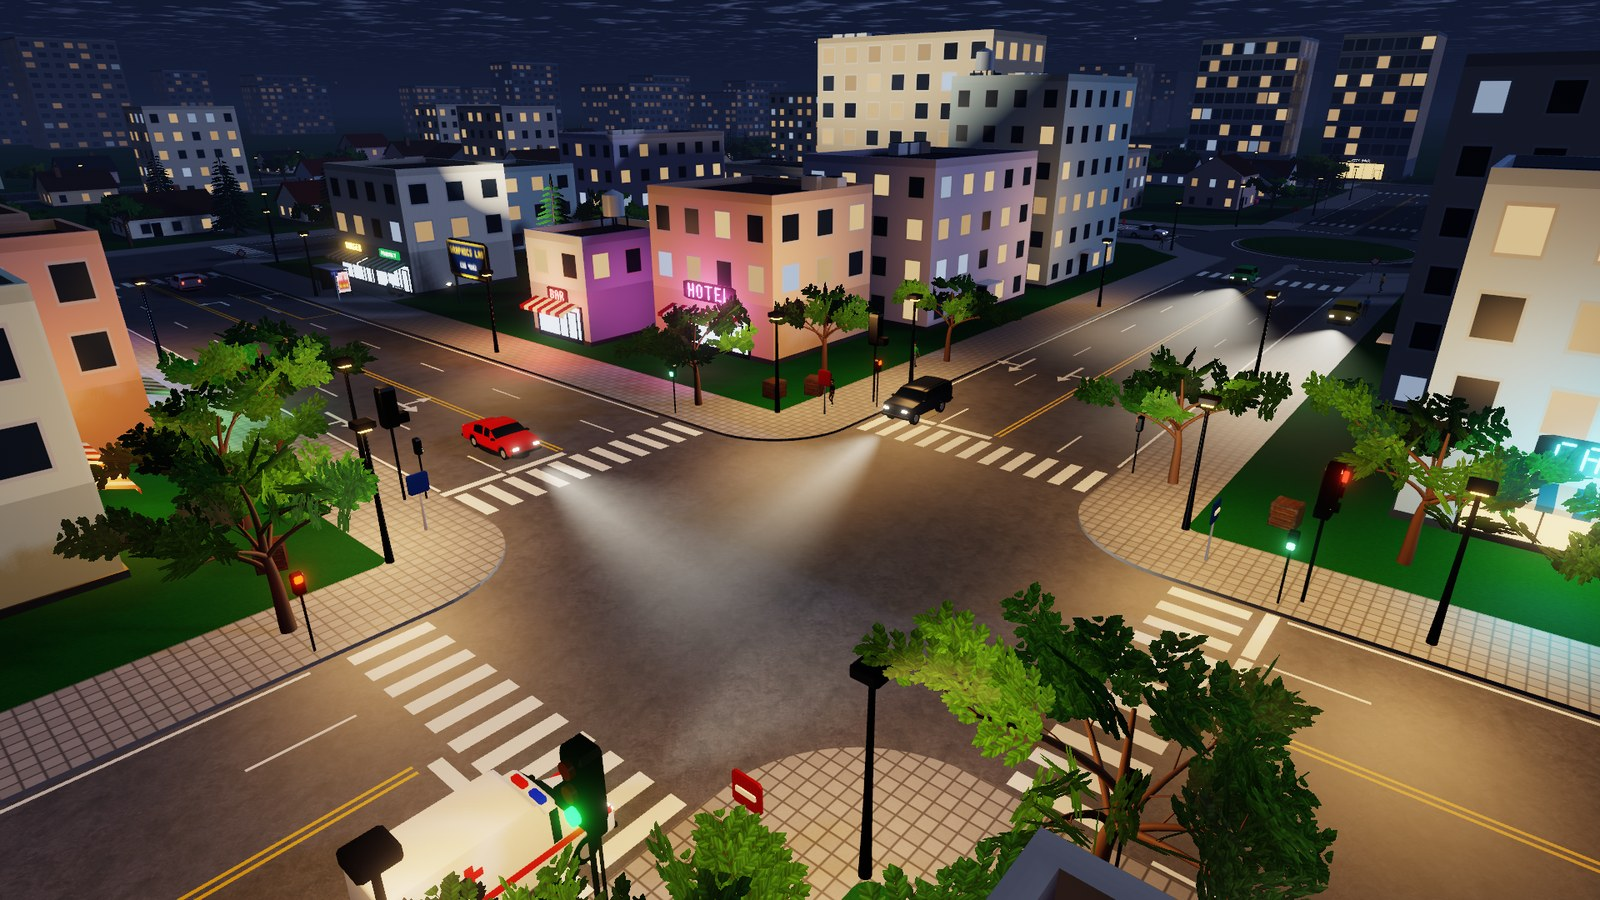
\includegraphics[width=\textwidth]{crossroads_night}};
  \begin{scope}[x={(img.south east)},y={(img.north west)}]
    \tikzset{lab/.style={fill=black!75,text=white,font=\scriptsize\bfseries,rounded corners=1pt,inner sep=2.5pt},
             pt/.style={-{Stealth[length=2mm]},very thick,yellow}}
    \node[lab] (a) at (0.20,0.93) {DIRECTIONAL: moonlight};
    \draw[pt] (a) -- (0.33,0.80);
    \node[lab] (b) at (0.83,0.75) {POINT: street lamp};
    \draw[pt] (b) -- (0.79,0.61);
    \node[lab] (c) at (0.45,0.30) {SPOT: headlights};
    \draw[pt] (c) -- (0.50,0.42);
    \node[lab] (d) at (0.12,0.78) {SPOT: billboard lamp};
    \draw[pt] (d) -- (0.28,0.71);
    \node[lab] (e) at (0.53,0.83) {EMISSIVE: neon};
    \draw[pt] (e) -- (0.45,0.68);
  \end{scope}
\end{tikzpicture}
\caption{All four light types in one frame: the central crossroads at 22:00.}
\end{figure}

\begin{calc}{point-light attenuation (the lab's constants)}
$A(d) = \dfrac{1}{k_c + k_l d + k_q d^2}$ with $k_c = 1$, $k_l = 0.09$, $k_q = 0.032$:
\begin{center}
\begin{tabular}{rcccc}
\toprule
$d$ (m) & 5.58 (under the lamp) & 10 & 15 & 22 (end of reach)\\ \midrule
$1 + 0.09d + 0.032d^2$ & 2.499 & 5.100 & 9.550 & 18.468\\
$A(d)$ & 0.400 & 0.196 & 0.105 & 0.054\\
\bottomrule
\end{tabular}
\end{center}
The light sits 5.58\,m above the foot of the post, so on the sidewalk straight under it $d = 5.58$\,m: $1 + 0.502 + 0.996 = 2.499$. At 22\,m the light is only 14\,\% of that, and a smooth window takes it to exactly zero, so the 32-light budget can swap lamps without any popping.
\end{calc}

\begin{calc}{spot-light cone}
Inside the inner cone the light is full, outside the outer cone it is zero, and between them
\[
\text{cone}(\theta) = \text{clamp}\left(\frac{\cos\theta - \cos\theta_{\text{out}}}{\cos\theta_{\text{in}} - \cos\theta_{\text{out}}}, 0, 1\right).
\]
Billboard lamp: $\cos 30^\circ = 0.866$, $\cos 42^\circ = 0.743$. A point $36^\circ$ off the axis: $(0.809 - 0.743)/(0.866 - 0.743) = 0.066/0.123 = 0.54$, just over half strength.\\
Headlights: $\cos 10^\circ = 0.985$, $\cos 26^\circ = 0.899$. At $18^\circ$: $(0.951 - 0.899)/(0.985 - 0.899) = 0.61$.
\end{calc}

\begin{calc}{diffuse and specular from the noon sun}
Noon: the sun is $59.2^\circ$ up, so on flat ground $\mathbf{N}\cdot\mathbf{L} = \sin 59.2^\circ = 0.859$. With the sun's colour $(1.54, 1.50, 1.38)$, the diffuse light on the ground is $(1.32, 1.29, 1.19)$, plus the sky ambient $(0.28, 0.34, 0.44)$.\\
Specular on paint ($\alpha = 64$) seen $5^\circ$ off the mirror direction: $\cos^{64} 5^\circ = 0.9962^{64} = 0.78$; at $15^\circ$ it is $0.9659^{64} = 0.11$, so the highlight is small and sharp. On grass ($\alpha = 6$) at $15^\circ$ it is $0.9659^6 = 0.81$: broad and, with a dim specular map, faint.
\end{calc}

\subsection{The sun and the moon}
The sun's position is that of a city at latitude $\phi = 40^\circ$\,N in late spring (declination $\delta = +10^\circ$). Its height $h$ at clock time $t$ comes from the hour angle $H = 15^\circ(t - 12.5)$:
\[
\sin h = \sin\phi\,\sin\delta + \cos\phi\,\cos\delta\,\cos H .
\]
\begin{calc}{the sun's height and the shadow length at each preset}
$\sin\phi\sin\delta = 0.6428 \times 0.1736 = 0.1116$ and $\cos\phi\cos\delta = 0.7660\times 0.9848 = 0.7544$. A pole 1\,m high throws a shadow $1/\tan h$ long.
\begin{center}\small\setlength{\tabcolsep}{4pt}
\begin{tabular}{@{}lcccccl@{}}
\toprule
Preset & $t$ & $H$ & $\sin h$ & $h$ & shadow/m & light \\ \midrule
Morning & 07:00 & $-82.5^\circ$ & $0.1116 + 0.7544(0.1305) = 0.2101$ & $12.1^\circ$ & 4.65\,m & sun, warm \\
Noon & 12:00 & $-7.5^\circ$ & $0.1116 + 0.7544(0.9914) = 0.8595$ & $59.3^\circ$ & 0.59\,m & sun, white \\
Afternoon & 15:30 & $45^\circ$ & $0.1116 + 0.7544(0.7071) = 0.6450$ & $40.2^\circ$ & 1.18\,m & sun, white \\
Evening & 18:30 & $90^\circ$ & $0.1116 + 0.7544(0) = 0.1116$ & $6.4^\circ$ & 8.90\,m & sun, orange \\
Night & 22:00 & --- & moon & $25^\circ$ & --- & moon, blue \\
\bottomrule
\end{tabular}
\end{center}
The program's own figures (\code{-{}-dimensions}, Table~\ref{tab:sun}) agree.
\end{calc}

\begin{table}[H]
\centering\small
\begin{tabular}{lccl}
\toprule
Preset & Light & Colour (linear RGB) & Height \\ \midrule
Morning 07:00 & sun & $(1.17, 0.81, 0.59)$ & $12^\circ$ \\
Noon 12:00 & sun & $(1.54, 1.50, 1.38)$ & $59^\circ$ \\
Afternoon 15:30 & sun & $(1.54, 1.50, 1.38)$ & $40^\circ$ \\
Evening 18:30 & sun & $(0.93, 0.56, 0.35)$ & $6^\circ$ \\
Night 22:00 & moon & $(0.08, 0.09, 0.16)$ & $25^\circ$ \\
\bottomrule
\end{tabular}
\caption{The directional light at each preset, printed by \code{-{}-dimensions}. The sun's colour is $\text{mix}(\text{day}, \text{sunset}, 0.75w)\times 1.6$, where $w$ grows as the sun gets low.}
\label{tab:sun}
\end{table}

\begin{figure}[H]
  \centering
  \begin{subfigure}{0.49\textwidth}\shot{\textwidth}{time_morning}\caption{Morning 07:00: long shadows to the west}\end{subfigure}\hfill
  \begin{subfigure}{0.49\textwidth}\shot{\textwidth}{time_noon}\caption{Noon 12:00: short shadows}\end{subfigure}\\[2mm]
  \begin{subfigure}{0.49\textwidth}\shot{\textwidth}{time_evening}\caption{Evening 18:30: orange sun, lamps on}\end{subfigure}\hfill
  \begin{subfigure}{0.49\textwidth}\shot{\textwidth}{time_night}\caption{Night 22:00: moon, lamps, lit windows}\end{subfigure}
  \caption{The directional light at four presets, from one view.}
\end{figure}

\subsection{Shadow maps}
The city is drawn from the light into two depth maps. A point is in shadow when it is farther from the light than the depth stored for it.
\begin{calc}{shadow-map resolution}
Near map: $2048\times2048$ over a 64\,m square round the camera, $64/2048 = 0.031$\,m (3\,cm) per texel. City map: $4096\times4096$ over the whole city, about 12\,cm per texel. The near map moves in steps of exactly one texel, so shadow edges never crawl. 16 depth-compare taps soften the edge.
\end{calc}

% =============================================================================
\section{Shading: Flat, Gouraud and Phong}
% =============================================================================

One shader pair does all three, chosen by \code{uShadingMode} (keys \code{1}, \code{2}, \code{3}):
\begin{itemize}
  \item \textbf{Flat} (mode 0): one normal per triangle, from the screen-space derivatives of the position, $\mathbf{N} = \text{normalize}\left(\frac{\partial\mathbf{P}}{\partial x}\times\frac{\partial\mathbf{P}}{\partial y}\right)$. Every face has one colour, so the facets show.
  \item \textbf{Gouraud} (mode 1): the lighting equation is evaluated in the \emph{vertex} shader (\code{scene.vert}) and the colours are interpolated across the triangle. Cheap, but a highlight smaller than a triangle is lost or smeared.
  \item \textbf{Phong} (mode 2): the \emph{normal} is interpolated and the lighting equation runs for every pixel. Smooth surfaces and sharp highlights.
\end{itemize}

\begin{calc}{why Gouraud loses a highlight}
Take an edge whose two vertices see the mirror direction $20^\circ$ away, while the middle of the edge sees it head on, with $\alpha = 58$. Gouraud: each vertex gives $\cos^{58} 20^\circ = 0.9397^{58} = 0.027$, so the middle of the edge gets $0.027$. Phong: the interpolated normal gives $\cos^{58} 0^\circ = 1$ in the middle. The highlight is 37 times brighter with Phong.
\end{calc}

\begin{figure}[H]
  \centering
  \begin{subfigure}{0.325\textwidth}\shot{\textwidth}{fountain_flat}\caption{Flat}\end{subfigure}\hfill
  \begin{subfigure}{0.325\textwidth}\shot{\textwidth}{fountain_gouraud}\caption{Gouraud}\end{subfigure}\hfill
  \begin{subfigure}{0.325\textwidth}\shot{\textwidth}{fountain_phong}\caption{Phong}\end{subfigure}
  \caption{The Bezier fountain in the three shading modes. Flat shows every facet of the basin; Gouraud and Phong are smooth, and Phong keeps the highlight on the column.}
\end{figure}

% =============================================================================
\section{Texture Mapping}
% =============================================================================

\code{Texture::fromFile(path, wrapS, wrapT, minFilter, magFilter)} follows the lab's \code{loadTexture}, so the wrapping and filtering are explicit at every use:

\begin{table}[H]
\centering\small
\begin{tabularx}{\textwidth}{@{}l l l X@{}}
\toprule
Texture & Wrap & Filter (min / mag) & Use \\ \midrule
\code{asphalt-photoreal.png} & \code{GL\_REPEAT} & \code{LINEAR\_MIPMAP\_LINEAR} / \code{LINEAR} & roads; one tile covers 80\,m of carriageway \\
grass, sidewalk & \code{GL\_REPEAT} & \code{LINEAR\_MIPMAP\_LINEAR} / \code{LINEAR} & lawns, pavements (procedural if the file is missing) \\
\code{container2.png} & \code{CLAMP\_TO\_EDGE} & \code{LINEAR\_MIPMAP\_LINEAR} / \code{LINEAR} & crate \textbf{diffuse} map \\
\code{container2\_specular.png} & \code{CLAMP\_TO\_EDGE} & \code{LINEAR\_MIPMAP\_LINEAR} / \code{LINEAR} & crate \textbf{specular} map (the metal edges shine, the wood does not) \\
leaf atlas (RGBA) & \code{CLAMP\_TO\_EDGE} & mipmapped & tree leaf cards, \textbf{alpha-tested} (\code{discard} below 0.5) \\
billboard faces & \code{CLAMP\_TO\_EDGE} & \code{LINEAR\_MIPMAP\_LINEAR} & $512\times256$ pictures drawn at start-up \\
\bottomrule
\end{tabularx}
\caption{Textures and their settings.}
\end{table}

\begin{calc}{texture repeat on the road}
Texture coordinates are world metres divided by the tile size: $u = x/80$. A road 400\,m long therefore has $u$ from 0 to 5, and \code{GL\_REPEAT} tiles the picture 5 times. With mipmaps, a road 200\,m away (where one pixel covers about 0.3\,m) reads a smaller copy of the picture instead of shimmering.
\end{calc}

\textbf{Windows without geometry.} A wall's texture coordinates count window bays across and storeys up. The fragment shader takes $\text{fract}(u)$ and $\text{fract}(v)$ to find the position inside one cell and draws a framed window there; at night a hash of the cell number decides whether that room is lit.

\begin{figure}[H]
  \centering
  \begin{subfigure}{0.49\textwidth}\shot{\textwidth}{street_level}\caption{Asphalt with \code{GL\_REPEAT}, sidewalks, windows}\end{subfigure}\hfill
  \begin{subfigure}{0.49\textwidth}\shot{\textwidth}{park_plaza}\caption{Alpha-tested leaf cards, paving, the plaza}\end{subfigure}
  \caption{Textures in the city.}
\end{figure}

% =============================================================================
\section{Bezier Curves and Surfaces}
% =============================================================================

A Bezier curve of degree $n$ with control points $\mathbf{P}_0\dots\mathbf{P}_n$ is
\[
\mathbf{B}(t) = \sum_{i=0}^{n} \binom{n}{i} (1-t)^{n-i} t^i\, \mathbf{P}_i, \qquad 0 \le t \le 1.
\]
\code{Mesh::makeBezierRevolution} uses the Lab~5 functions \code{nCr} and the Bernstein sum to turn a list of (radius, height) control points into a profile, and sweeps the profile round the $y$ axis to make a solid: the vertex at profile point $(r, y)$ and angle $\phi$ is $(r\cos\phi,\ y,\ r\sin\phi)$.

\begin{table}[H]
\centering\small
\begin{tabular}{@{}lll@{}}
\toprule
Object & Control points $(r, y)$ in metres & Degree \\ \midrule
Fountain basin & $(0,0), (1.90,0.06), (1.45,0.32), (1.90,0.78), (2.10,1.06)$ & 4 \\
Fountain column & $(0.46,0), (0.20,0.72), (0.22,1.32), (0.78,1.70), (0.86,1.96), (0.12,2.06)$ & 5 \\
Lamp post & $(0.17,0), (0.10,1.60), (0.085,4.00), (0.075,5.60)$ & 3 \\
Bin & $(0.22,0), (0.27,0.5), (0.30,0.92), (0.32,0.98), (0,1.0)$ & 4 \\
Bollard & $(0.11,0), (0.10,0.7), (0.11,0.85), (0.07,0.98), (0,1.0)$ & 4 \\
Water-tank roof & $(1.08,0), (0.6,0.28), (0,0.5)$ & 2 \\
Plaza monument & $(0.55,0), (0.22,0.6), (0.2,1.4), (0.75,2.0), (0.5,2.7), (0.05,3.4)$ & 5 \\
\bottomrule
\end{tabular}
\caption{Control points written in the source (\code{Scene.cpp}, \code{PropRenderer.cpp}).}
\end{table}

\begin{calc}{a point on the fountain basin at $t = 0.5$}
$n = 4$; the Bernstein weights at $t = 0.5$ are $\binom{4}{i}/16 = (1, 4, 6, 4, 1)/16$.
\begin{align*}
r &= \tfrac{1}{16}\big(1(0) + 4(1.90) + 6(1.45) + 4(1.90) + 1(2.10)\big) = \tfrac{26.0}{16} = 1.625\text{ m},\\
y &= \tfrac{1}{16}\big(1(0) + 4(0.06) + 6(0.32) + 4(0.78) + 1(1.06)\big) = \tfrac{6.34}{16} = 0.396\text{ m}.
\end{align*}
The curve starts at the centre of the floor $(0, 0)$ and ends at the rim, $2.10$\,m out and $1.06$\,m up: a basin $4.2$\,m across. It is swept with 22 profile steps and 28 around, $22\times28 = 616$ quads.
\end{calc}

\textbf{Curves in 3D.} Tree trunks and branches are tubes swept along cubic Bezier curves in 3D (de Casteljau's construction), and vehicle bodies are straight runs joined by Bezier corners, swept across the width.

\begin{figure}[H]
  \centering
  \begin{subfigure}{0.49\textwidth}\shot{\textwidth}{tour_billboard}\caption{Bezier lamp posts, trees; the billboard}\end{subfigure}\hfill
  \begin{subfigure}{0.49\textwidth}\shot{\textwidth}{roundabout_r2}\caption{Roundabout R2: arcs and lamp posts}\end{subfigure}
  \caption{Bezier surfaces of revolution and curves in the city.}
\end{figure}

% =============================================================================
\section{Objects and Their Dimensions}\label{sec:dimensions}
% =============================================================================

All sizes are in metres. They are printed by the program itself with \code{OpenGLMiniProject.exe -{}-dimensions}, from the same tables the program draws with, so they cannot disagree with the picture. Sizes that are only numbers inside the drawing code are given with the file they come from.

\subsection{Vehicles}
\begin{table}[H]
\centering\footnotesize\setlength{\tabcolsep}{4pt}
\begin{tabular}{@{}lcccccccc@{}}
\toprule
Kind & Class & Length & Width & Height & Wheelbase & Wheel $r$ & Cruise km/h & Acc./brake m/s$^2$\\ \midrule
Sedan & car & 4.70 & 1.84 & 1.45 & 2.75 & 0.33 & 31 & 1.60 / 2.20\\
Hatchback (yours) & car & 4.06 & 1.80 & 1.48 & 2.75 & 0.32 & 30 & 1.60 / 2.20\\
SUV & car & 4.80 & 1.88 & 1.74 & 2.75 & 0.38 & 30 & 1.50 / 2.20\\
Taxi & car & 4.70 & 1.84 & 1.45 & 2.75 & 0.33 & 32 & 1.70 / 2.30\\
Police car & car & 4.84 & 1.88 & 1.48 & 2.75 & 0.33 & 32 & 1.80 / 2.40\\
Van & van & 5.20 & 1.88 & 2.25 & 2.90 & 0.36 & 29 & 1.30 / 2.00\\
Pickup & van & 5.40 & 1.88 & 1.82 & 2.90 & 0.38 & 30 & 1.40 / 2.10\\
Ambulance & van & 5.50 & 1.88 & 2.60 & 2.90 & 0.37 & 32 & 1.40 / 2.10\\
Box truck & truck & 7.90 & 2.30 & 3.30 & 3.40 & 0.48 & 27 & 1.00 / 1.80\\
City bus & bus & 12.00 & 2.54 & 3.15 & 5.90 & 0.50 & 27 & 0.95 / 1.70\\
Motorbike & car & 2.10 & 0.80 & 1.55 & 1.40 & 0.31 & 34 & 2.20 / 2.60\\
\bottomrule
\end{tabular}
\caption{Vehicle sizes (\code{VehicleTypes.cpp}; wheel radius from \code{VehicleRenderer.cpp}).}
\end{table}
The traffic plans junctions with one outline per size class (half length $\times$ half width): car $2.45\times0.94$, van $2.75\times0.94$, truck $3.95\times1.15$, bus $6.00\times1.27$. Every kind fits inside its class outline (checked by \code{-{}-self-test}).

\subsection{Roads and junctions}
\begin{table}[H]
\centering\small
\begin{tabularx}{\textwidth}{@{}l X@{}}
\toprule
City & 400 $\times$ 400 (grid of junctions every 100); walkable square 600 $\times$ 600 \\
Lanes & 2 each way, 3.50 wide (lane centres 1.75 and 5.25 from the centre line); road 14.0 kerb to kerb \\
Sidewalk & 4.5 wide; kerb 0.15 high (road surface at $y = 0.06$, sidewalk at $y = 0.21$) \\
Crossroads & kerb corner radius 5.0; zebra band 12.6--15.4 from the centre; stop line at 16.0 \\
Bends & centre-line radius 20.0 \\
Roundabouts & island radius 9.5; circulating lane radius 13.0; outer kerb radius 17.0; entry and exit arcs 8.0; zebra 25.0--28.0 from the centre \\
Network & 19 junctions: 2 signalised crossroads, 3 signalised T-junctions, 7 give-way T-junctions, 2 roundabouts, 5 bends; 28 roads; 54 zebra crossings; 252 routes; 1614 conflict zones \\
\bottomrule
\end{tabularx}
\caption{Road dimensions (\code{RoadNetwork.h}).}
\end{table}

\subsection{Buildings}
\begin{table}[H]
\centering\small
\begin{tabular}{@{}lrccccc@{}}
\toprule
Style & Count & Front width & Depth & Height & Storeys & Storey height\\ \midrule
Shop row & 43 & 7.0--21.9 & 9.0--12.0 & 4.8--14.7 & 1--4 & 3.3 (ground floor 4.2)\\
Flats & 39 & 14.0--19.9 & 11.1--12.9 & 9.9--19.2 & 3--6 & 3.1\\
Office tower & 20 & 16.2--21.6 & 15.4--18.6 & 27.0--48.6 & 7--13 & 3.6\\
Hotel & 4 & 22.7--26.3 & 12.0--13.2 & 24.3--30.7 & 7--9 & 3.2\\
House & 51 & 9.0--10.5 & 8.0--9.4 & 2.9--5.8 & 1--2 & 2.9\\
Warehouse & 7 & 24.6--33.7 & 16.3--21.1 & 7.6 & 1 & 7.0\\ \midrule
Skyline (400--700 out) & 90 & 18.3--40.0 & 18.3--39.9 & 17.6--78.8 & 5--23 & 3.4\\
\bottomrule
\end{tabular}
\caption{The 164 buildings of the city and the skyline (\code{WorldCity.cpp}). Shop fronts: 103, 5.8--10.0 wide, 43 with neon signs. Neon signs: 47, letters 0.62--1.40 high.}
\end{table}

\begin{calc}{height of a building from its storeys}
A block of flats with 5 storeys: $5 \times 3.1 = 15.5$\,m plus a 0.6\,m parapet gives $16.1$\,m, within the 9.9--19.2 range. An office tower of 12 storeys: $12\times3.6 = 43.2$\,m, plus a glazed lobby.
\end{calc}

\subsection{Trees, street furniture and signals}
\begin{table}[H]
\centering\small
\begin{tabularx}{\textwidth}{@{}lr X l@{}}
\toprule
Object & Count & Size & Source \\ \midrule
Broadleaf tree & 171 & height 5.9--8.1, crown radius 3.4--5.6 & \code{TreeGenerator.cpp}\\
Conifer & 72 & height 7.5--10.4, crown radius 2.5--3.3 & \code{TreeGenerator.cpp}\\
Palm & 12 & height 6.1--7.4, crown radius 3.2--4.0 & \code{TreeGenerator.cpp}\\
Street lamp & 182 + 12 & Bezier post 5.60 high, 0.17 radius at the foot; head $0.75\times0.28\times0.75$ at 5.75 & \code{Scene.cpp}\\
Traffic signal & 17 & pole $0.13\times4.50\times0.13$; housing $0.72\times1.85\times0.55$ at 4.45; 3 lenses 0.38 across; arrow box $0.46\times0.46\times0.50$ & \code{Scene.cpp}\\
Walk signal & 34 & a short pole at each end of a signalised crossing & \code{Scene.cpp}\\
Give-way sign & 15 & Bezier post, red plate $0.70\times0.70$ at 2.15 & \code{Scene.cpp}\\
Billboard & 8 & panel $6.0\times3.0$, underside 2.6 above the ground & \code{World.h}\\
Bus shelter & 4 & $3.6$ long $\times$ 1.5 deep $\times$ 2.5 high & \code{World.h}\\
Bench & 30 & seat $1.8\times0.45$ high, back 0.27 behind & \code{PropRenderer.cpp}\\
Bin & 22 & 1.0 high, radius 0.32 & \code{PropRenderer.cpp}\\
Planter & 40 & trough $1.7\times0.6\times0.8$ with two shrubs & \code{PropRenderer.cpp}\\
Bollard & 4 & 1.0 high, radius 0.11 & \code{PropRenderer.cpp}\\
Picnic table & 3 & top $1.8\times0.8$ at 0.75 & \code{PropRenderer.cpp}\\
50 km/h sign & 12 & post 2.4, disc radius 0.4 & \code{PropRenderer.cpp}\\
Crate & 6 & $1.05$ cube & \code{Scene.cpp}\\
Parked car & 49 & as the vehicle table & \code{WorldCity.cpp}\\
Fountain & 1 & basin 4.2 across, 1.06 high; column 2.06 high on it & \code{Scene.cpp}\\
Pond & 1 & ellipse $25.0\times16.0$ & \code{WorldCity.cpp}\\
Petrol-station canopy & 1 & $16.0\times10.0$, 5.2 high & \code{World.h}\\
Plaza monument & 1 & pedestal $2.6^2\times1.0$ + $1.8^2\times0.6$, flame 3.4 high & \code{PropRenderer.cpp}\\
\bottomrule
\end{tabularx}
\caption{Trees, furniture and signals.}
\end{table}

\subsection{People and the camera}
People are 1.56--1.90\,m tall (height $= 1.56 + 0.34\,u_1(0.4 + 0.6u_2)$ for random $u_1, u_2$), built with the proportions of a 1.75\,m figure and scaled: thigh 0.455, shin 0.445, torso 0.44, upper arm 0.29, forearm 0.26. You on foot are 1.78\,m tall with your eyes at 1.65\,m. The camera's field of view is $55^\circ$ (free, top, chase), $68^\circ$ in a car and $62^\circ$ on foot; the far plane is at 1200\,m.

\begin{figure}[H]
  \centering
  \begin{subfigure}{0.49\textwidth}\shot{\textwidth}{bus_stop}\caption{Bus (12\,m) at a shelter ($3.6\times1.5\times2.5$)}\end{subfigure}\hfill
  \begin{subfigure}{0.49\textwidth}\shot{\textwidth}{petrol_station}\caption{Petrol station, lamp posts, a person}\end{subfigure}\\[2mm]
  \begin{subfigure}{0.49\textwidth}\shot{\textwidth}{houses}\caption{Houses, shop row, lamp posts}\end{subfigure}\hfill
  \begin{subfigure}{0.49\textwidth}\shot{\textwidth}{walk_signal}\caption{Traffic signal, walk light, give-way sign}\end{subfigure}
  \caption{Objects at street level, to compare their sizes.}
\end{figure}

% =============================================================================
\section{Traffic and Digital Signals}
% =============================================================================

\subsection{Conflict zones: collision-free by construction}
For every pair of routes through a junction, both routes are sampled every 25\,cm and a car-sized box (plus a 30\,cm margin) is placed at each sample. Every pair of positions where the two boxes overlap is marked, and each connected patch of marks is a \textbf{conflict zone}. The city has 252 routes and 1614 zones.

A car \textbf{commits} to a junction only when, in one check, its signal allows it, the car in front has committed, there is room beyond the junction, no crossing car holds a claim on a zone on its way, and no car with priority could arrive within 3.5\,s. It then \textbf{claims every zone on its way at once} and releases each one as it leaves it. A committed car never waits for a claim, so there is no deadlock; two cars on crossing routes are never in a shared zone together, so there is no collision.

\subsection{The digital signals}
Every signalised junction has its own controller. Each axis gets: a protected \textbf{left-turn arrow} (only when someone waits to turn left) $\rightarrow$ \textbf{green} $\rightarrow$ \textbf{yellow} $\rightarrow$ 2.5\,s \textbf{all-red}. Green is actuated: it ends early once its queue is empty and someone waits across, and never runs past 16\,s while someone waits. Walkers get a green WALK figure, then a flashing red one.

\begin{figure}[H]
  \centering
  \begin{subfigure}{0.49\textwidth}\shot{\textwidth}{tour_red_light}\caption{Your car (yellow) waits at red, left arrow lit}\end{subfigure}\hfill
  \begin{subfigure}{0.49\textwidth}\shot{\textwidth}{tour_green_light}\caption{Green: it drives on}\end{subfigure}\\[2mm]
  \begin{subfigure}{0.49\textwidth}\shot{\textwidth}{tour_people}\caption{People crossing on WALK}\end{subfigure}\hfill
  \begin{subfigure}{0.49\textwidth}\shot{\textwidth}{crossroads_day}\caption{The central crossroads X0}\end{subfigure}
  \caption{Digital traffic signals and pedestrian crossings.}
\end{figure}

\subsection{Car following: the Intelligent Driver Model}
\[
a = a_{\max}\left[1 - \left(\frac{v}{v_0}\right)^4 - \left(\frac{s^*}{s}\right)^2\right], \qquad s^* = s_0 + vT + \frac{v\,\Delta v}{2\sqrt{a_{\max}b}} .
\]
\begin{calc}{a sedan approaching a stopped car}
Sedan: $v_0 = 8.6$\,m/s, $a_{\max} = 1.6$, $b = 2.2$, $T = 1.1$\,s, $s_0 = 2.0$\,m. It drives at $v = 8$\,m/s towards a stopped car $s = 30$\,m ahead ($\Delta v = 8$).
\begin{align*}
s^* &= 2.0 + 8(1.1) + \frac{8 \times 8}{2\sqrt{1.6\times2.2}} = 2.0 + 8.8 + \frac{64}{3.752} = 27.86\text{ m},\\
a &= 1.6\left[1 - (8/8.6)^4 - (27.86/30)^2\right] = 1.6\,[1 - 0.749 - 0.862] = -0.98\text{ m/s}^2 .
\end{align*}
It brakes gently now, well below the comfortable $2.2$\,m/s$^2$. Corners ahead are braked for from $v^2 = v_c^2 + 2ad$.
\end{calc}

% =============================================================================
\section{Weather}
% =============================================================================

Clear, Cloudy or Rain (\code{K} or a click); every change blends over 10\,s. Clouds are a sheet 1.5\,km up, shaped by six octaves of noise, and throw drifting shadows. Rain is up to 5,000 instanced streaks in one draw call. Wet surfaces get darker and glossier, and puddles mirror the sky by Schlick's Fresnel law:
\[
F(\theta) = F_0 + (1 - F_0)(1 - \cos\theta)^5, \qquad F_0 = 0.02 .
\]
\begin{calc}{how much a puddle mirrors}
Looking straight down ($\theta = 0^\circ$): $F = 0.02$, only 2\,\%. At $60^\circ$: $0.02 + 0.98(0.5)^5 = 0.051$. At $80^\circ$ (a street seen from eye height a few metres ahead): $0.02 + 0.98(1 - 0.174)^5 = 0.02 + 0.98(0.386) = 0.40$. This is why wet roads shine most in the distance.
\end{calc}

\begin{figure}[H]
  \centering
  \begin{subfigure}{0.325\textwidth}\shot{\textwidth}{weather_clear}\caption{Clear}\end{subfigure}\hfill
  \begin{subfigure}{0.325\textwidth}\shot{\textwidth}{weather_cloudy}\caption{Cloudy}\end{subfigure}\hfill
  \begin{subfigure}{0.325\textwidth}\shot{\textwidth}{weather_rain}\caption{Rain}\end{subfigure}
  \caption{The three kinds of weather at 15:30, same view.}
\end{figure}

% =============================================================================
\section{Ray Tracing (Bonus)}
% =============================================================================

OpenGL~3.3 has no ray-tracing hardware, and tracing rays through the whole city in software would not hold 60\,FPS. So the project uses \textbf{partial ray tracing}: after the city is drawn, rays are marched through its \textbf{depth buffer}, which holds the nearest surface under every pixel. Clicking the ray-tracing button (or \code{F3}) asks ``RAY TRACING ON?'' in the middle of the screen; \emph{Yes} turns it on.

\begin{table}[H]
\centering\small
\begin{tabularx}{\textwidth}{@{}l l X@{}}
\toprule
Effect & Resolution & How \\ \midrule
Reflections & half & A ray reflected off every mirror-like surface is marched in 32 growing steps until it passes behind the depth buffer, then refined by 5 halvings \\
Ambient occlusion & half & 12 points in the half ball above each surface; those behind the depth buffer are shut in \\
Contact shadows & half & 10 steps up the sunbeam, under 1\,m: shadows under tyres, feet, kerbs \\
Soft shadows (PCSS) & full & A search finds how far above a point its casters are; the edge is blurred that wide \\
Sun shafts & quarter & Open sky near a low sun is gathered along the line to the sun \\
\bottomrule
\end{tabularx}
\caption{The ray-tracing passes.}
\end{table}

\subsection{How a reflection ray is marched}
\begin{enumerate}
  \item From the depth $z$ of pixel $(x, y)$, rebuild the view-space position $\mathbf{P} = z\,\cdot P^{-1}(x_{ndc}, y_{ndc}, 1)$ and the normal $\mathbf{N}$ from neighbouring depths.
  \item Reflect the view ray: $\mathbf{R} = \mathbf{V} - 2(\mathbf{V}\cdot\mathbf{N})\mathbf{N}$.
  \item Step along $\mathbf{R}$: $\mathbf{Q}_k = \mathbf{P} + t_k \mathbf{R}$, with a first step of $0.1 + 0.01\,z$ metres (longer for far surfaces), each step $1.12\times$ the last. Project $\mathbf{Q}_k$ to the screen and compare its depth with the depth buffer there.
  \item When the ray first passes \emph{behind} the stored surface, halve the last step 5 times (binary search) to find the hit, then read the colour there.
  \item Fade the result near the screen's edges and where the ray points back at the camera; multiply by the surface's mirror strength (Fresnel).
\end{enumerate}

\begin{calc}{the reach of the reflection ray}
For a wet road $z = 20$\,m away the first step is $0.1 + 0.01(20) = 0.3$\,m, and each step is $1.12\times$ the last. After 32 steps the ray has gone
\[
0.3\,\frac{1.12^{32} - 1}{1.12 - 1} = 0.3 \times \frac{37.58 - 1}{0.12} = 0.3 \times 304.8 = 91.4\text{ m}.
\]
A step counts as a hit when the ray is behind the stored surface by less than $\max(0.4,\ 1.5\times\text{step})$; otherwise it passed behind a whole object. The last step is then halved 5 times, which finds the hit to within $1/2^5 = 1/32$ of that step: at the 20th step ($0.3\times1.12^{19} = 2.6$\,m) that is 8\,cm. (\code{shaders/ssr.frag})
\end{calc}

\begin{figure}[H]
  \centering
  \begin{subfigure}{0.49\textwidth}\shot{\textwidth}{rt_off_rain_night}\caption{Ray tracing OFF}\end{subfigure}\hfill
  \begin{subfigure}{0.49\textwidth}\shot{\textwidth}{rt_on_rain_night}\caption{Ray tracing ON: bus lights, neon and shops mirrored}\end{subfigure}
  \caption{Night in the rain on the shopping street.}
\end{figure}

\begin{figure}[H]
  \centering
  \begin{subfigure}{0.49\textwidth}\shot{\textwidth}{tour_rt_question}\caption{The ``RAY TRACING ON?'' question}\end{subfigure}\hfill
  \begin{subfigure}{0.49\textwidth}\shot{\textwidth}{tour_reflections_1}\caption{Lamps, signals and neon reflected}\end{subfigure}\\[2mm]
  \begin{subfigure}{0.49\textwidth}\shot{\textwidth}{rt_off_noon}\caption{Noon, OFF}\end{subfigure}\hfill
  \begin{subfigure}{0.49\textwidth}\shot{\textwidth}{rt_on_noon}\caption{Noon, ON: occlusion and soft shadows}\end{subfigure}
  \caption{Turning ray tracing on, and its effects.}
\end{figure}

\textbf{Limits.} Rays can only hit what is on screen: a building behind the camera never shows in a puddle, and reflections fade towards the screen's edges. That is why it is called \emph{partial} ray tracing.

\subsection{Cost}
Measured at 1080p on the RTX 3050 laptop GPU, the passes take 0.6--0.9\,ms in all (reflections 0.2--0.3, occlusion and contact shadows 0.2--0.35, sun shafts 0.1, composite 0.2), and the soft shadows add 0.2--0.35\,ms: about 1\,ms of the 13.9\,ms frame. The heaviest view goes from 9.3--9.4 to 10.0--10.3\,ms and every tested view stays at a steady 72\,FPS.

% =============================================================================
\section{Performance and Testing}
% =============================================================================

\subsection{Frame rate}
\begin{table}[H]
\centering\small
\begin{tabular}{@{}llcccc@{}}
\toprule
View & Weather & FPS & 99th percentile & Worst & GPU \\ \midrule
Whole city, noon & Cloudy & 72 & 14.7 ms & 15.0 ms & 5.6 ms\\
Whole city, night & Rain & 72 & 14.8 ms & 16.3 ms & 5.6 ms\\
Shopping street, night & Rain & 72 & 15.1 ms & 18.6 ms & 6.8 ms\\
Street level, noon & Rain & 72 & 15.0 ms & 32.4 ms & 5.2 ms\\
Your driver's seat, noon & Rain & 72 & 14.9 ms & 18.7 ms & 5.5 ms\\
G and ST, evening & Clear & 72 & 15.0 ms & 22.5 ms & 7.8 ms\\
G and ST, evening & Cloudy & 72 & 14.7 ms & 16.8 ms & 9.8 ms\\
G and ST, evening, ray tracing on & Cloudy & 72 & --- & --- & 10.0--10.3 ms\\
\bottomrule
\end{tabular}
\caption{1920$\times$1080, 80 people, 400 measured frames per view. 72\,FPS is every second refresh of the 144\,Hz screen (steady pacing).}
\end{table}

\subsection{Automatic tests}
All tests run from the command line without a window. Every one passed on the final build:
\begin{table}[H]
\centering\small
\begin{tabularx}{\textwidth}{@{}l X@{}}
\toprule
Test & Result \\ \midrule
\code{-{}-self-test} & 16,282 network, route, body, conflict, signal and bus-line checks; 575 sidewalk checks; every building, tree and prop on the lawn and clear of the road: \textbf{PASS} \\
\code{-{}-soak 30 seed} (clear) & Seeds 1--16, 30 simulated minutes each: \textbf{0 overlaps}, 0 vehicle--person touches, 0 starts against the lights; longest stop 54.1\,s (limit 60), longest wait 75.3\,s (limit 90), 2766--2830 routes driven: \textbf{16/16 PASS} \\
\code{-{}-soak} in the rain & Seeds 1--16: 0 overlaps; longest stop 50.4\,s, longest wait 72.0\,s, 2496--2562 routes: \textbf{16/16 PASS} \\
\code{-{}-motion-test} & Judder with interpolation 0.0007--0.0013 (limit 0.01) at 144, 60 and 75\,Hz: \textbf{PASS} \\
\code{-{}-light-test} & 236 lights, 109,008 frames, largest change of a light in one frame 0.011 (limit 0.1): \textbf{PASS} \\
\code{-{}-sun-test} & Every glide smooth ($\le 2.46^\circ$ per frame), shadows stable within 0.00024 texel: \textbf{PASS} \\
\code{-{}-weather-test} & Every change 10\,s, smooth; wet after 41\,s, puddles full after 96\,s: \textbf{PASS} \\
\code{-{}-walk-test} & Feet slide under 1\,\% of the distance, never sink: \textbf{PASS} \\
\code{-{}-player-test} & Crashes never enter walls; 1.5 laps among 36 AI cars, 0 hits: \textbf{PASS} \\
\bottomrule
\end{tabularx}
\caption{Test results (logs in \code{delivery/report/logs/}).}
\end{table}

% =============================================================================
\section{User Guide}
% =============================================================================

Build \code{OpenGLMiniProject.slnx} as x64 Release in Visual Studio and run it from the project folder.

\begin{longtable}{@{}>{\ttfamily}p{38mm} p{118mm}@{}}
\toprule
\normalfont\bfseries Key & \bfseries Action \\ \midrule
\endhead
W A S D, Q / E & Move the free camera (or drive / walk); down / up \\
Mouse & Look around \\
C & Lock the camera onto your car (or you on foot) \\
Arrows, Space, Shift & Drive, handbrake, boost \\
V / B & Chase view $\leftrightarrow$ driver view / look back \\
F & Get out of the car / back in \\
M & Top view of the whole city \\
Tab / Shift+Tab & Follow the next AI car / the next person \\
1 2 3 & \textbf{Flat / Gouraud / Phong shading} \\
O, [ ], click & \textbf{Time presets} Morning, Noon, Afternoon, Evening, Night; one hour back / on \\
T, Y / N, L & Automatic day--night; noon / night; night lights \\
K, click & \textbf{Weather}: Clear $\rightarrow$ Cloudy $\rightarrow$ Rain \\
F3, click & \textbf{Ray tracing} (asks ``RAY TRACING ON?'') \\
F2 & Shadows high / low / off \\
P, R, H & Pause, reset, help panel \\
F5 F6 F7 F11 & Frame graph, resolution, pacing, fullscreen \\
Esc & Exit \\
\bottomrule
\end{longtable}

% =============================================================================
\section{Conclusion and Future Work}
% =============================================================================

The project shows every topic of the lab in one working city: 3D transformations (MVP matrices, rotated routes, hierarchical vehicles), the illumination model with directional, point, spot and emissive lights, flat, Gouraud and Phong shading, texture mapping, Bezier curves and surfaces, and partial ray tracing for the bonus. The traffic is collision-free by construction and obeys digital signals; 32 half-hour soak tests found no collision. The city holds 72\,FPS at 1080p with ray tracing on.

\textbf{Future work:} full hardware ray tracing (Vulkan or DirectX Raytracing) so that off-screen objects appear in reflections; storms and fog; more junction types and a larger city; imported building models.

\subsection*{References}
\begin{enumerate}[label={[\arabic*]}]
  \item J. de Vries, \emph{Learn OpenGL}, \url{https://learnopengl.com} (lighting, shadow mapping, SSAO).
  \item D. Hearn, M. P. Baker, W. Carithers, \emph{Computer Graphics with OpenGL}, 4th ed., Pearson.
  \item M. Treiber, A. Hennecke, D. Helbing, ``Congested traffic states in empirical observations and microscopic simulations'', \emph{Physical Review E} 62, 2000 (the Intelligent Driver Model).
  \item M. McGuire, M. Mara, ``Efficient GPU Screen-Space Ray Tracing'', \emph{Journal of Computer Graphics Techniques} 3(4), 2014.
  \item R. Fernando, ``Percentage-Closer Soft Shadows'', SIGGRAPH Sketches, 2005.
  \item CSE 4102 lab sheets 1--5 (transformations, 3D drawing, illumination, textures, Bezier curves).
\end{enumerate}

% =============================================================================
\appendix
\section{Screenshot Gallery}
% =============================================================================

\begin{figure}[H]
  \centering
  \begin{subfigure}{0.49\textwidth}\shot{\textwidth}{tour_city}\caption{Flying over the city}\end{subfigure}\hfill
  \begin{subfigure}{0.49\textwidth}\shot{\textwidth}{ring_road}\caption{The park and the ring road}\end{subfigure}\\[2mm]
  \begin{subfigure}{0.49\textwidth}\shot{\textwidth}{tour_evening}\caption{Evening over the car park}\end{subfigure}\hfill
  \begin{subfigure}{0.49\textwidth}\shot{\textwidth}{tour_night_city}\caption{The city at night}\end{subfigure}\\[2mm]
  \begin{subfigure}{0.49\textwidth}\shot{\textwidth}{tour_neon_street}\caption{Neon street at night}\end{subfigure}\hfill
  \begin{subfigure}{0.49\textwidth}\shot{\textwidth}{shopping_night}\caption{Shopping street at night}\end{subfigure}
  \caption{Views of the city.}
\end{figure}

\begin{figure}[H]
  \centering
  \begin{subfigure}{0.49\textwidth}\shot{\textwidth}{street_level_night}\caption{Street level at night}\end{subfigure}\hfill
  \begin{subfigure}{0.49\textwidth}\shot{\textwidth}{sky_night}\caption{Night sky and the Grand Hotel}\end{subfigure}\\[2mm]
  \begin{subfigure}{0.49\textwidth}\shot{\textwidth}{rain_night_driver}\caption{Driver view in the rain, wipers}\end{subfigure}\hfill
  \begin{subfigure}{0.49\textwidth}\shot{\textwidth}{tour_reflections_2}\caption{Reflections on the wet road}\end{subfigure}\\[2mm]
  \begin{subfigure}{0.49\textwidth}\shot{\textwidth}{people_waiting}\caption{People waiting at X0}\end{subfigure}\hfill
  \begin{subfigure}{0.49\textwidth}\shot{\textwidth}{zebra}\caption{A zebra at a give-way junction}\end{subfigure}
  \caption{Night, rain and people.}
\end{figure}

\section{Rebuilding the Deliverables}
\begin{tabularx}{\textwidth}{@{}>{\ttfamily\small}l X@{}}
\toprule
\normalfont\bfseries Command & \bfseries Makes \\ \midrule
OpenGLMiniProject.exe -{}-dimensions & every object's size (this report's tables) \\
sh delivery/figures/capture\_all.sh & the screenshots (\code{-{}-capture}) \\
python delivery/figures/make\_figures.py & the JPEG figures \\
python delivery/video/make\_video.py & the 2-minute demo video \\
pdflatex report.tex (twice) & this report \\
python delivery/slides/build\_slides.py & the 10 slides \\
\bottomrule
\end{tabularx}

\end{document}
